\documentclass{article}
\usepackage[utf8]{inputenc}
\usepackage{hyperref}
\usepackage{algorithm}
\usepackage{algorithmicx}
\usepackage[table]{xcolor}
\usepackage{algpseudocode}
\usepackage{authblk}
\usepackage{graphicx}
\usepackage[margin=0.70in]{geometry}
\usepackage{listings}
\usepackage{indentfirst}


\title{Homework 2-2: Parallelizing a Particle Simulation with MPI}
\author{Andrew Chen}
\author{Xuan Jiang}
\author{Brian Park}
\affil{UC Berkeley, Computer Science 267}
\date{March 2022}

\begin{document}

\maketitle
\section{Introduction}
We used variety of techniques to optimize the problem of parallelizing $n$-body particle simulation on the Cori KNL node. We used the $O(n)$ solution from our previous homework to accelerate it with MPI (Message Passing Interface) \cite{mpi}.

\section{MPI}

\subsection{Data Structures}
Used the same binning idea that we derived from homework 2-1. To be more specific:

\begin{itemize}
	\item \verb|typedef vector<particle_t*> bin_t| \\
	      This holds pointers to all of the particles that lie within a bin.
	\item \verb|bin_t* bins| \\
	      This holds the vector of bins stored in row-major order.
\end{itemize}


\subsection{Design Choice}
For MPI, it was much harder to implement due to explicit communication. We mainly took use of communication primitives such as \verb|MPI_Isend| and \verb|MPI_Irecv|. We only used this to explicitly send or receive neighboring particles when computing \verb|apply_force()|. Note that we only focused on moving between rows in a 1D layout. We found moving bins by a grid, in a 2D layout is much harder to implement. Given more time, we would've tackled the 2D layout. For rebinning, we used \verb|MPI_Allgather| and \verb|MPI_Allgatherv|. We didn't want to deal with implementing additional data structure such as creating a ghost buffer or halo zone. Rather, we kept it simple and implemented All-to-All communication so that we can just rebin. We would need to synchronize before moving to the next step anyways, so this was the safest approach as well in order to achieve correctness. This is actually the same approach we took in OpenMP solution, but due to communication bottleneck in a distributed system, implementing explicit send and receive primitives may have been the more appropriate and tedious programming model. Due to the time it takes to debug and the performance we would achieve, we just stuck to this implementation. For \verb|gather_for_save()|, we implemented \verb|MPI_Gather| and \verb|MPI_Gatherv|. The reason why we used two gather version is because the sizes to collect are not uniform, so first we must calculate the size so that we can concatenate them properly in the second call to gather that uses the \verb|MPI_Gatherv| version, indicating variable length buffer. This is a many-to-one collective communication primitive and was necessary to communicate everything to the driver node to check for correctness when we save to output. The most difficult part of implementing gather was getting displacement right and how to collectively communicate data from different processes.

We make sure that particles are stored in bins. The number of bins is fixed, which is why we use an array of bins. The bins themselves change in size each simulation as they move around, which is why we use \verb|std::vector|.

\section{Experimental Results}
We evaluate the results of $n$-body particle simulations with random seed set to $42$ to make results reproducible.

\begin{figure}[H]
	\centering
	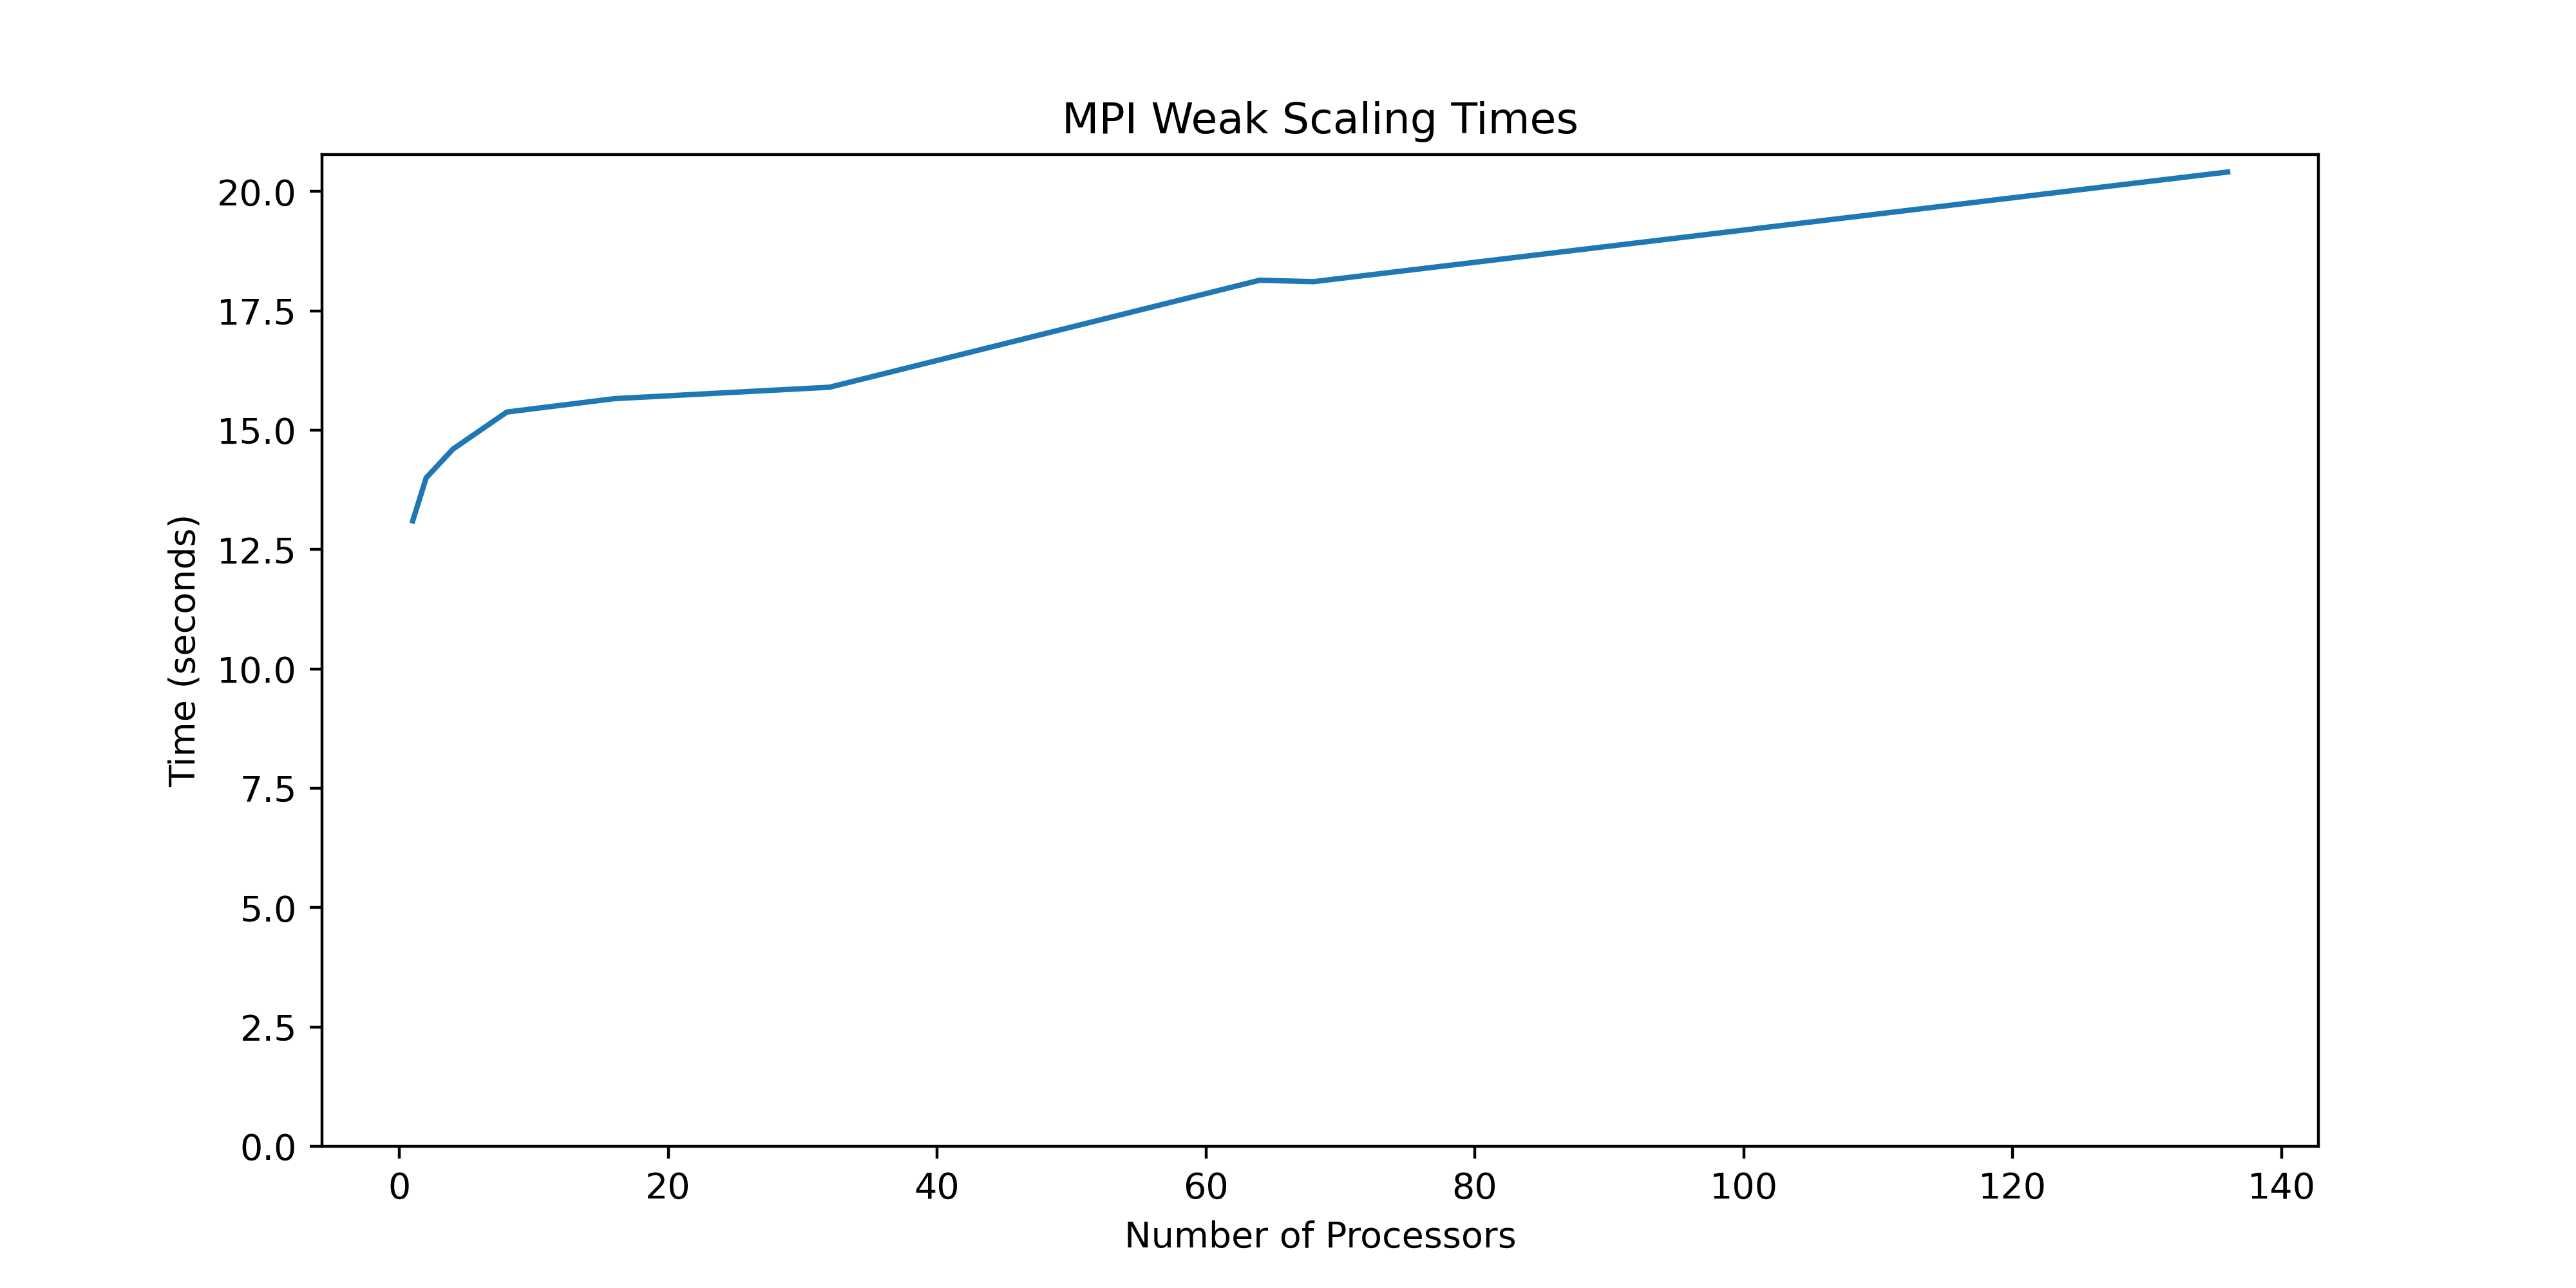
\includegraphics[width=6in]{figures/mpi_weak_scaling_times.png}
	\caption{MPI Weak Scaling}
	\label{fig:mpi-weak-scaling}
\end{figure}

Figure \ref{fig:mpi-weak-scaling} shows the weak scaling of MPI as it scales with 10000 particles per processor. We extend this to two nodes when running 136 processors (2 nodes $\times$ 68 processors).

\begin{figure}[H]
	\centering
	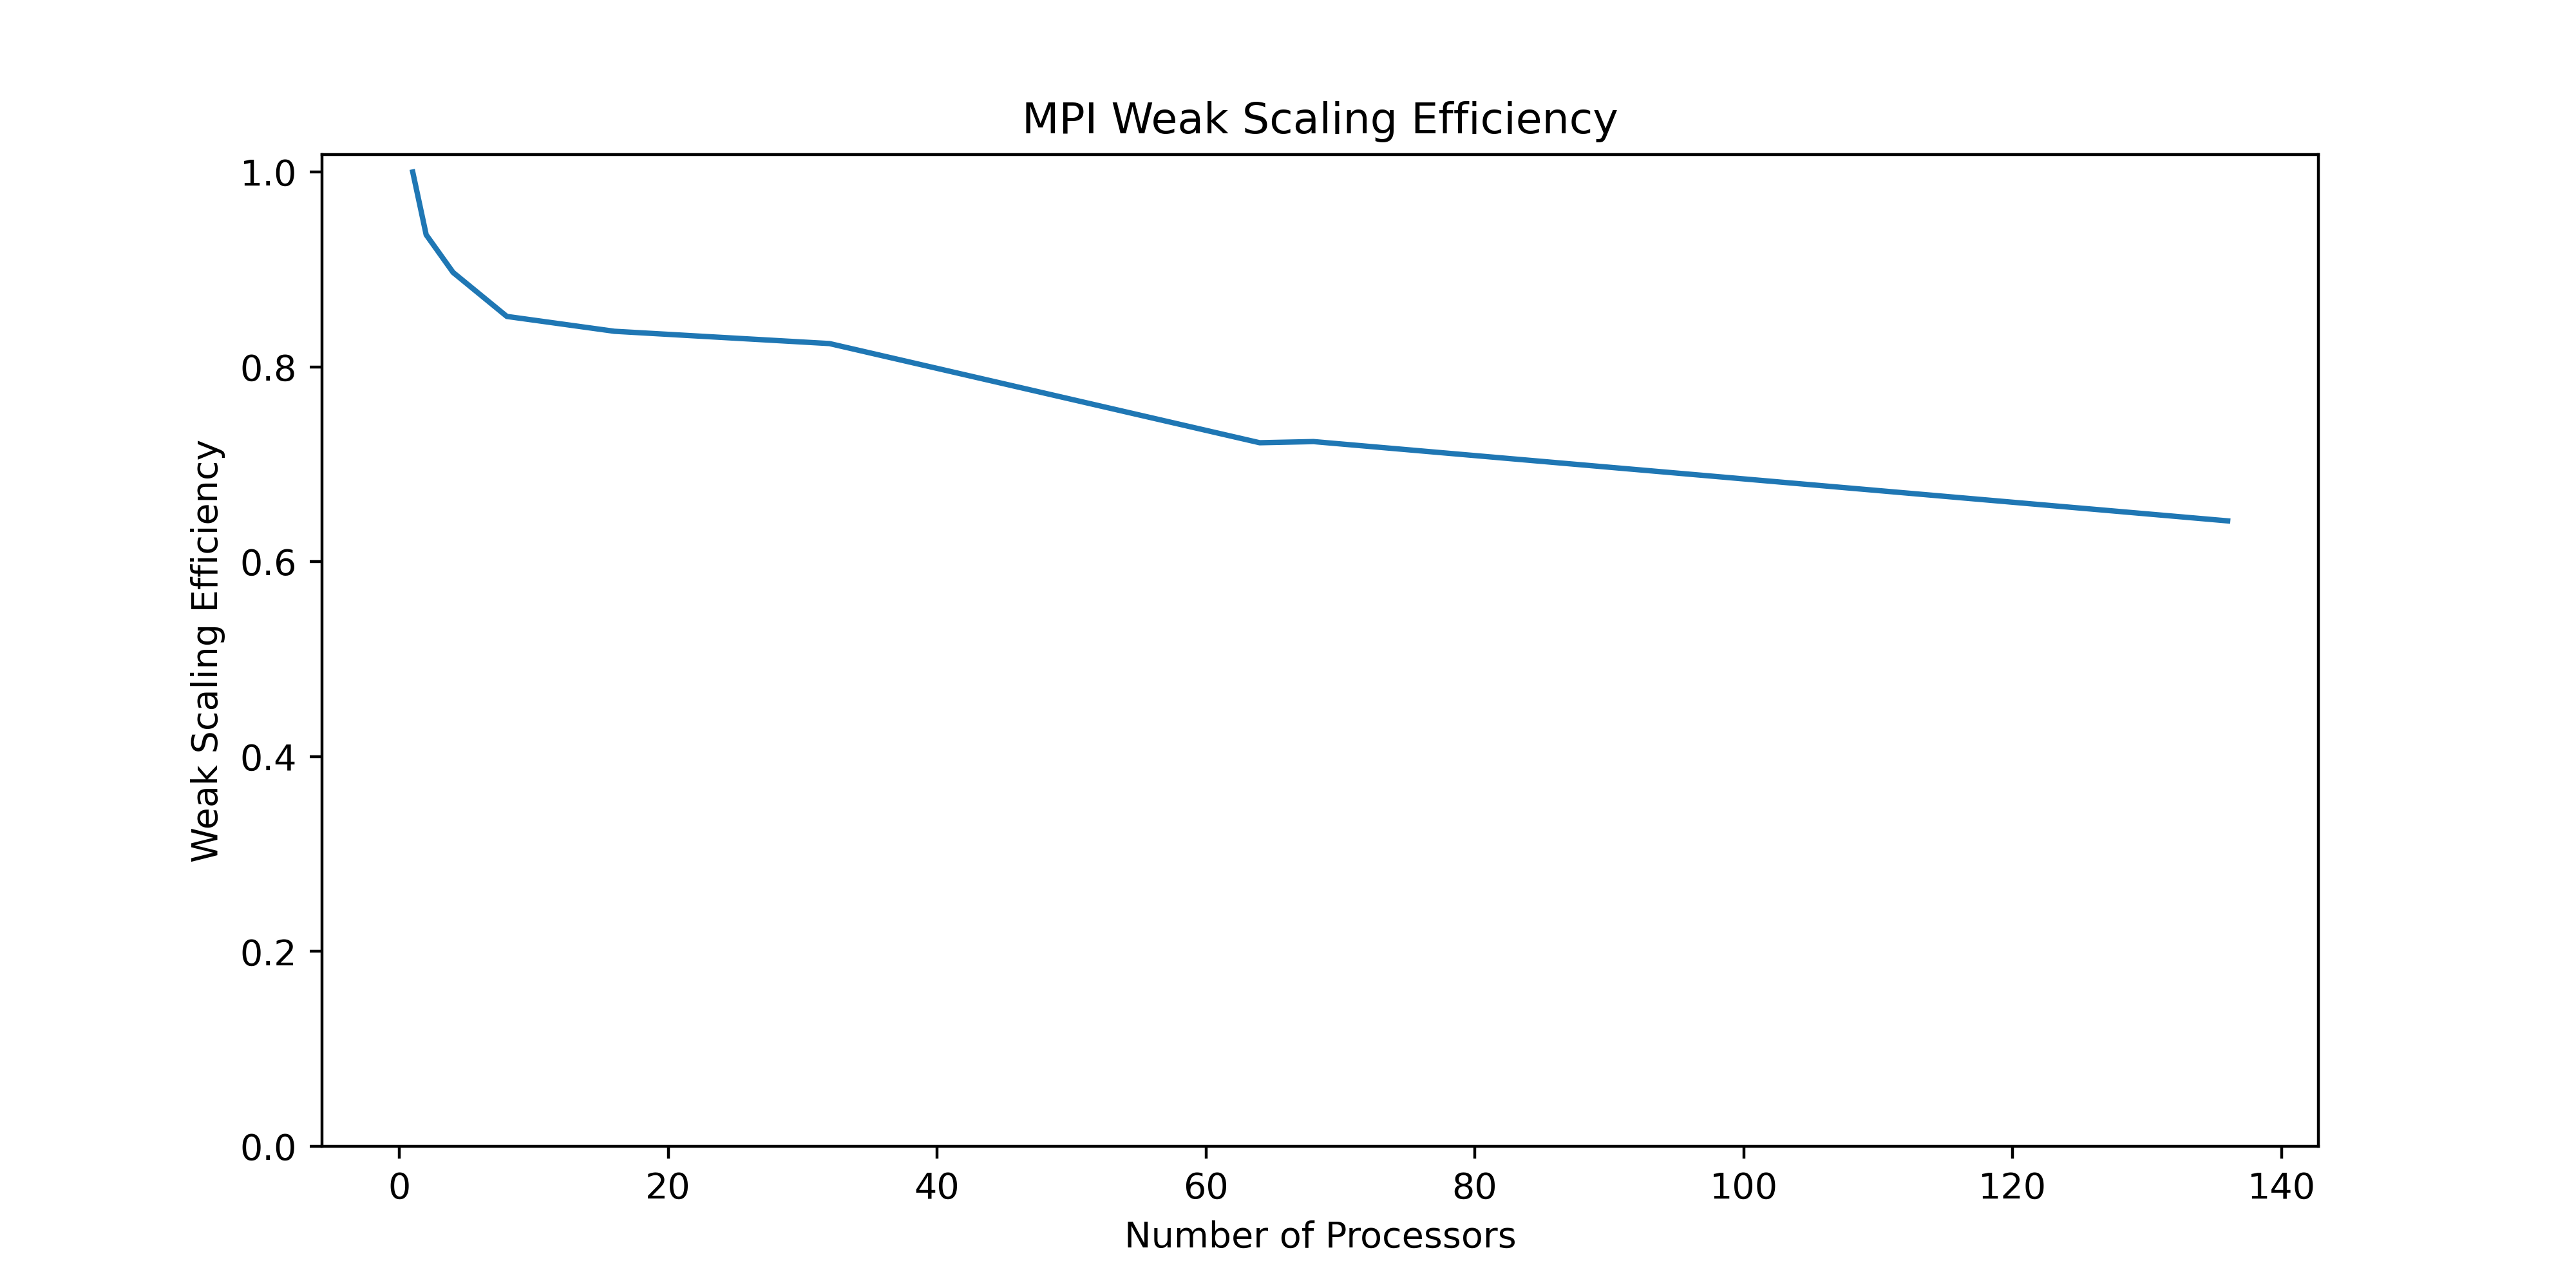
\includegraphics[width=6in]{figures/mpi_weak_scaling_efficiency.png}
	\caption{MPI Weak Scaling Efficiency}
	\label{fig:mpi-weak-scaling-efficiency}
\end{figure}

Figure \ref{fig:mpi-weak-scaling-efficiency} shows the weak scaling efficiency of MPI. We see that it somewhat sustains performance. When jumping to two processors, it has 93.6\% efficiency and then gradually drops to 64.2\% efficiency when scaled up to 136 processors.

\begin{figure}[H]
	\centering
	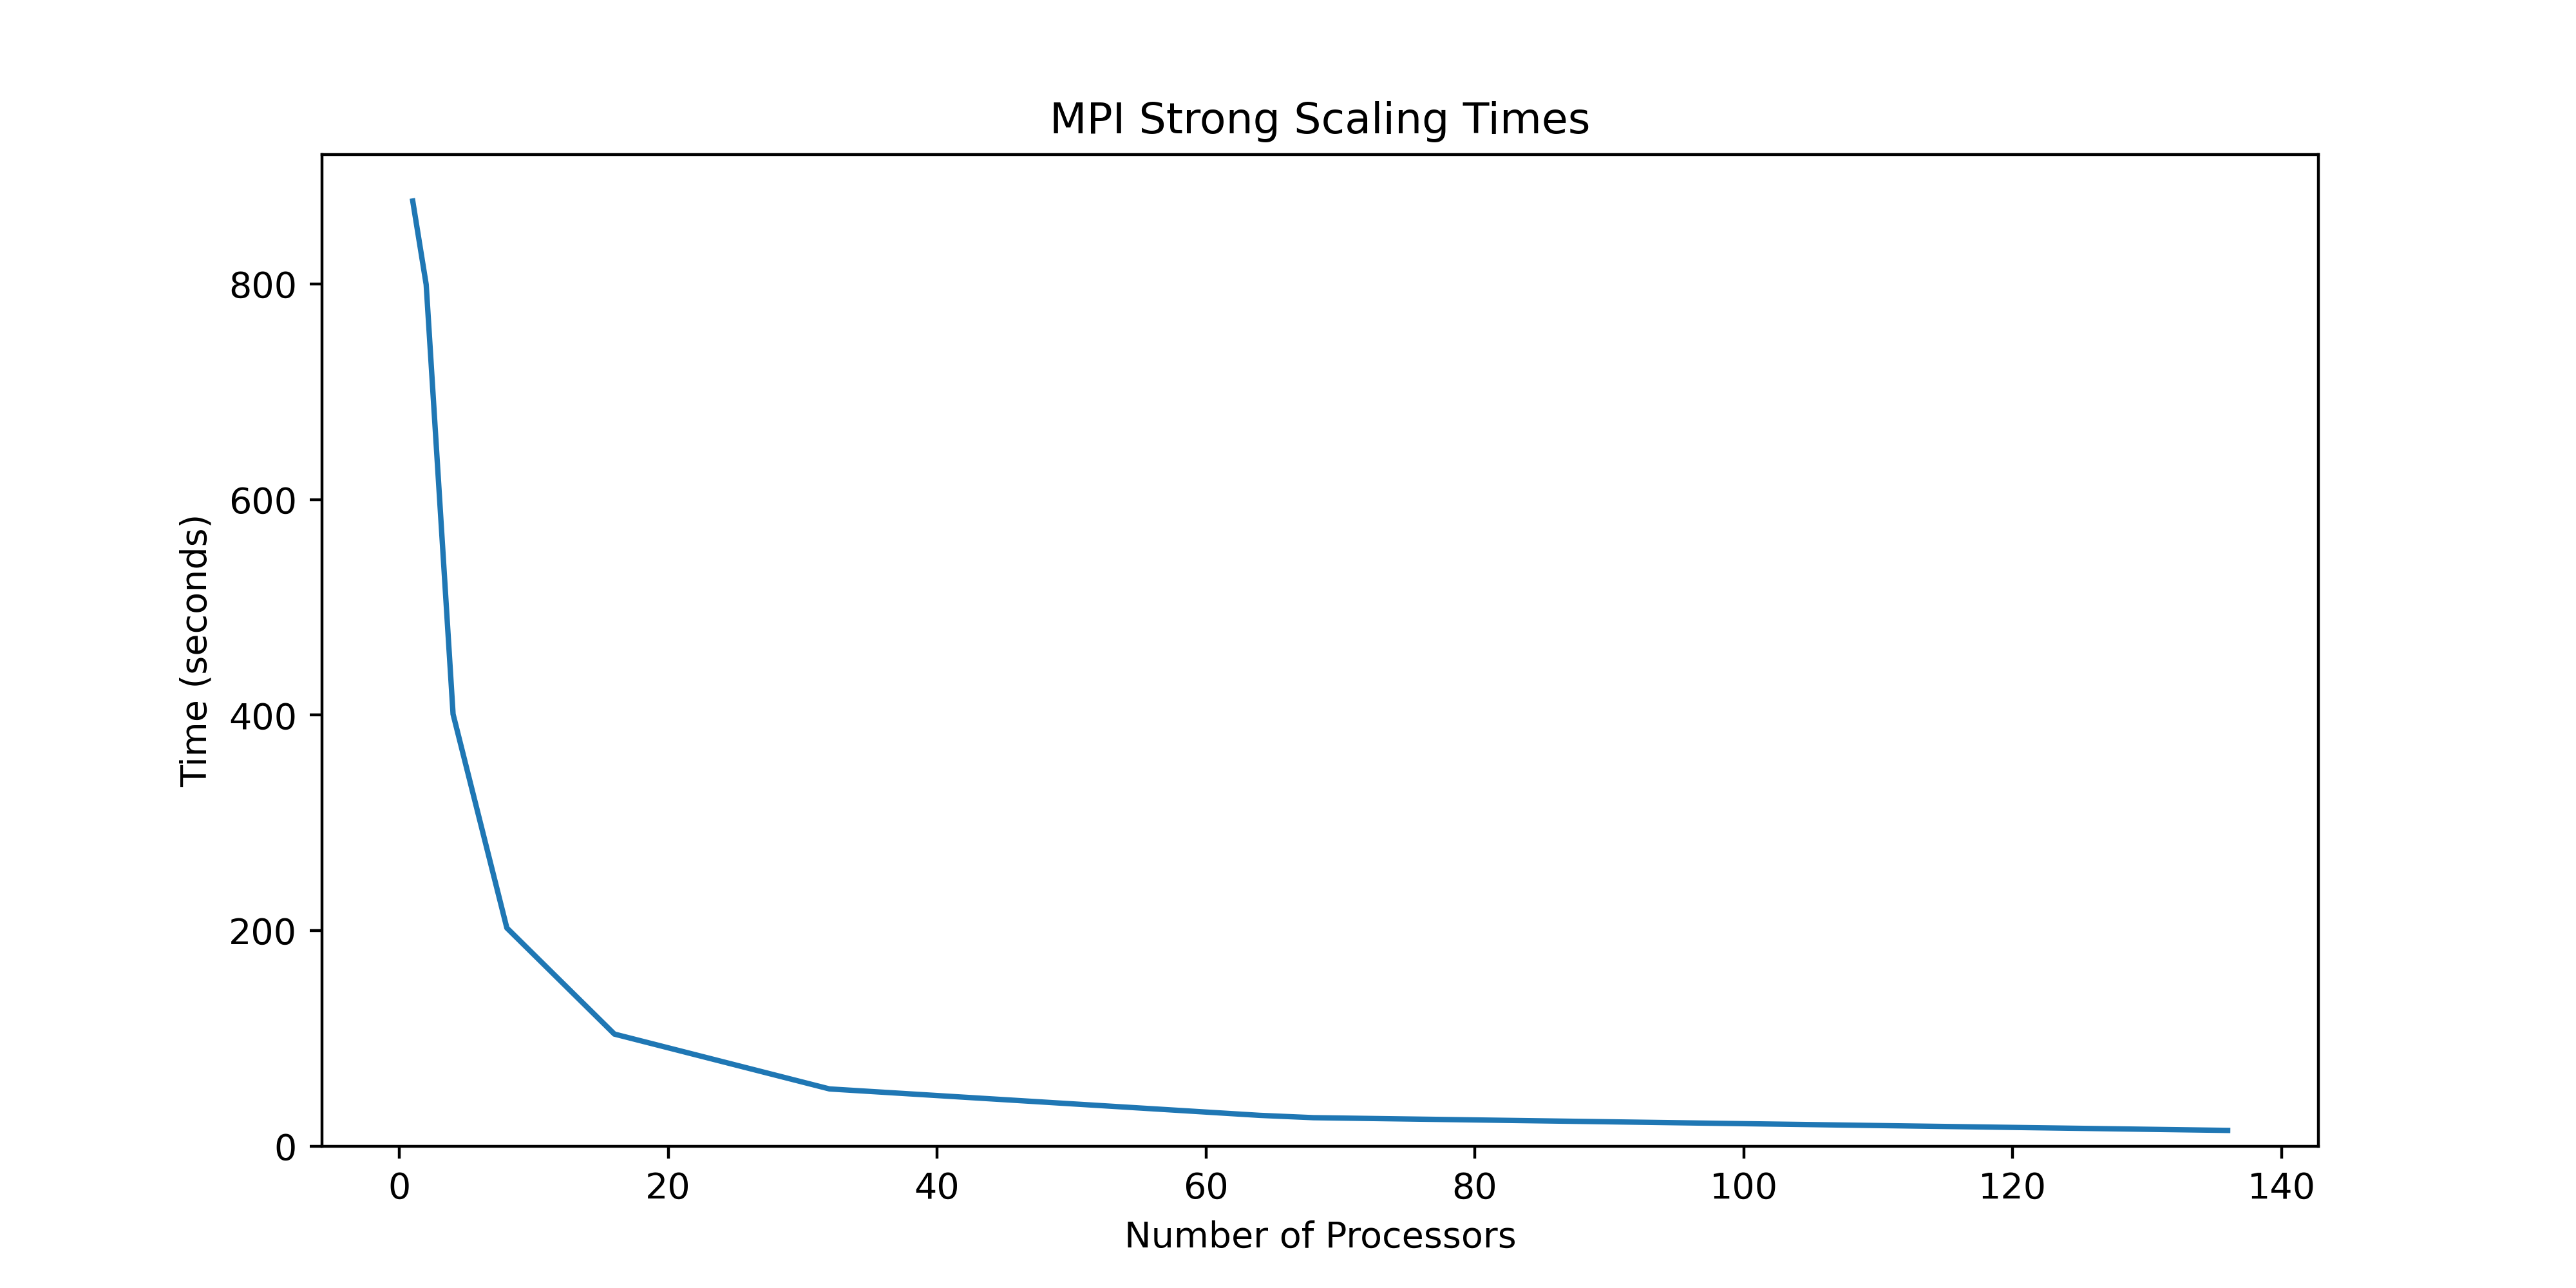
\includegraphics[width=6in]{figures/mpi_strong_scaling_times.png}
	\caption{MPI Strong Scaling}
	\label{fig:mpi-strong-scaling}
\end{figure}

Figure \ref{fig:mpi-strong-scaling} shows the strong scaling of our simulation with MPI for 1 million particles. We see that it decreases as expected. It reaches 14.8 seconds when all of the 136 cores are utilized.

\begin{figure}[H]
	\centering
	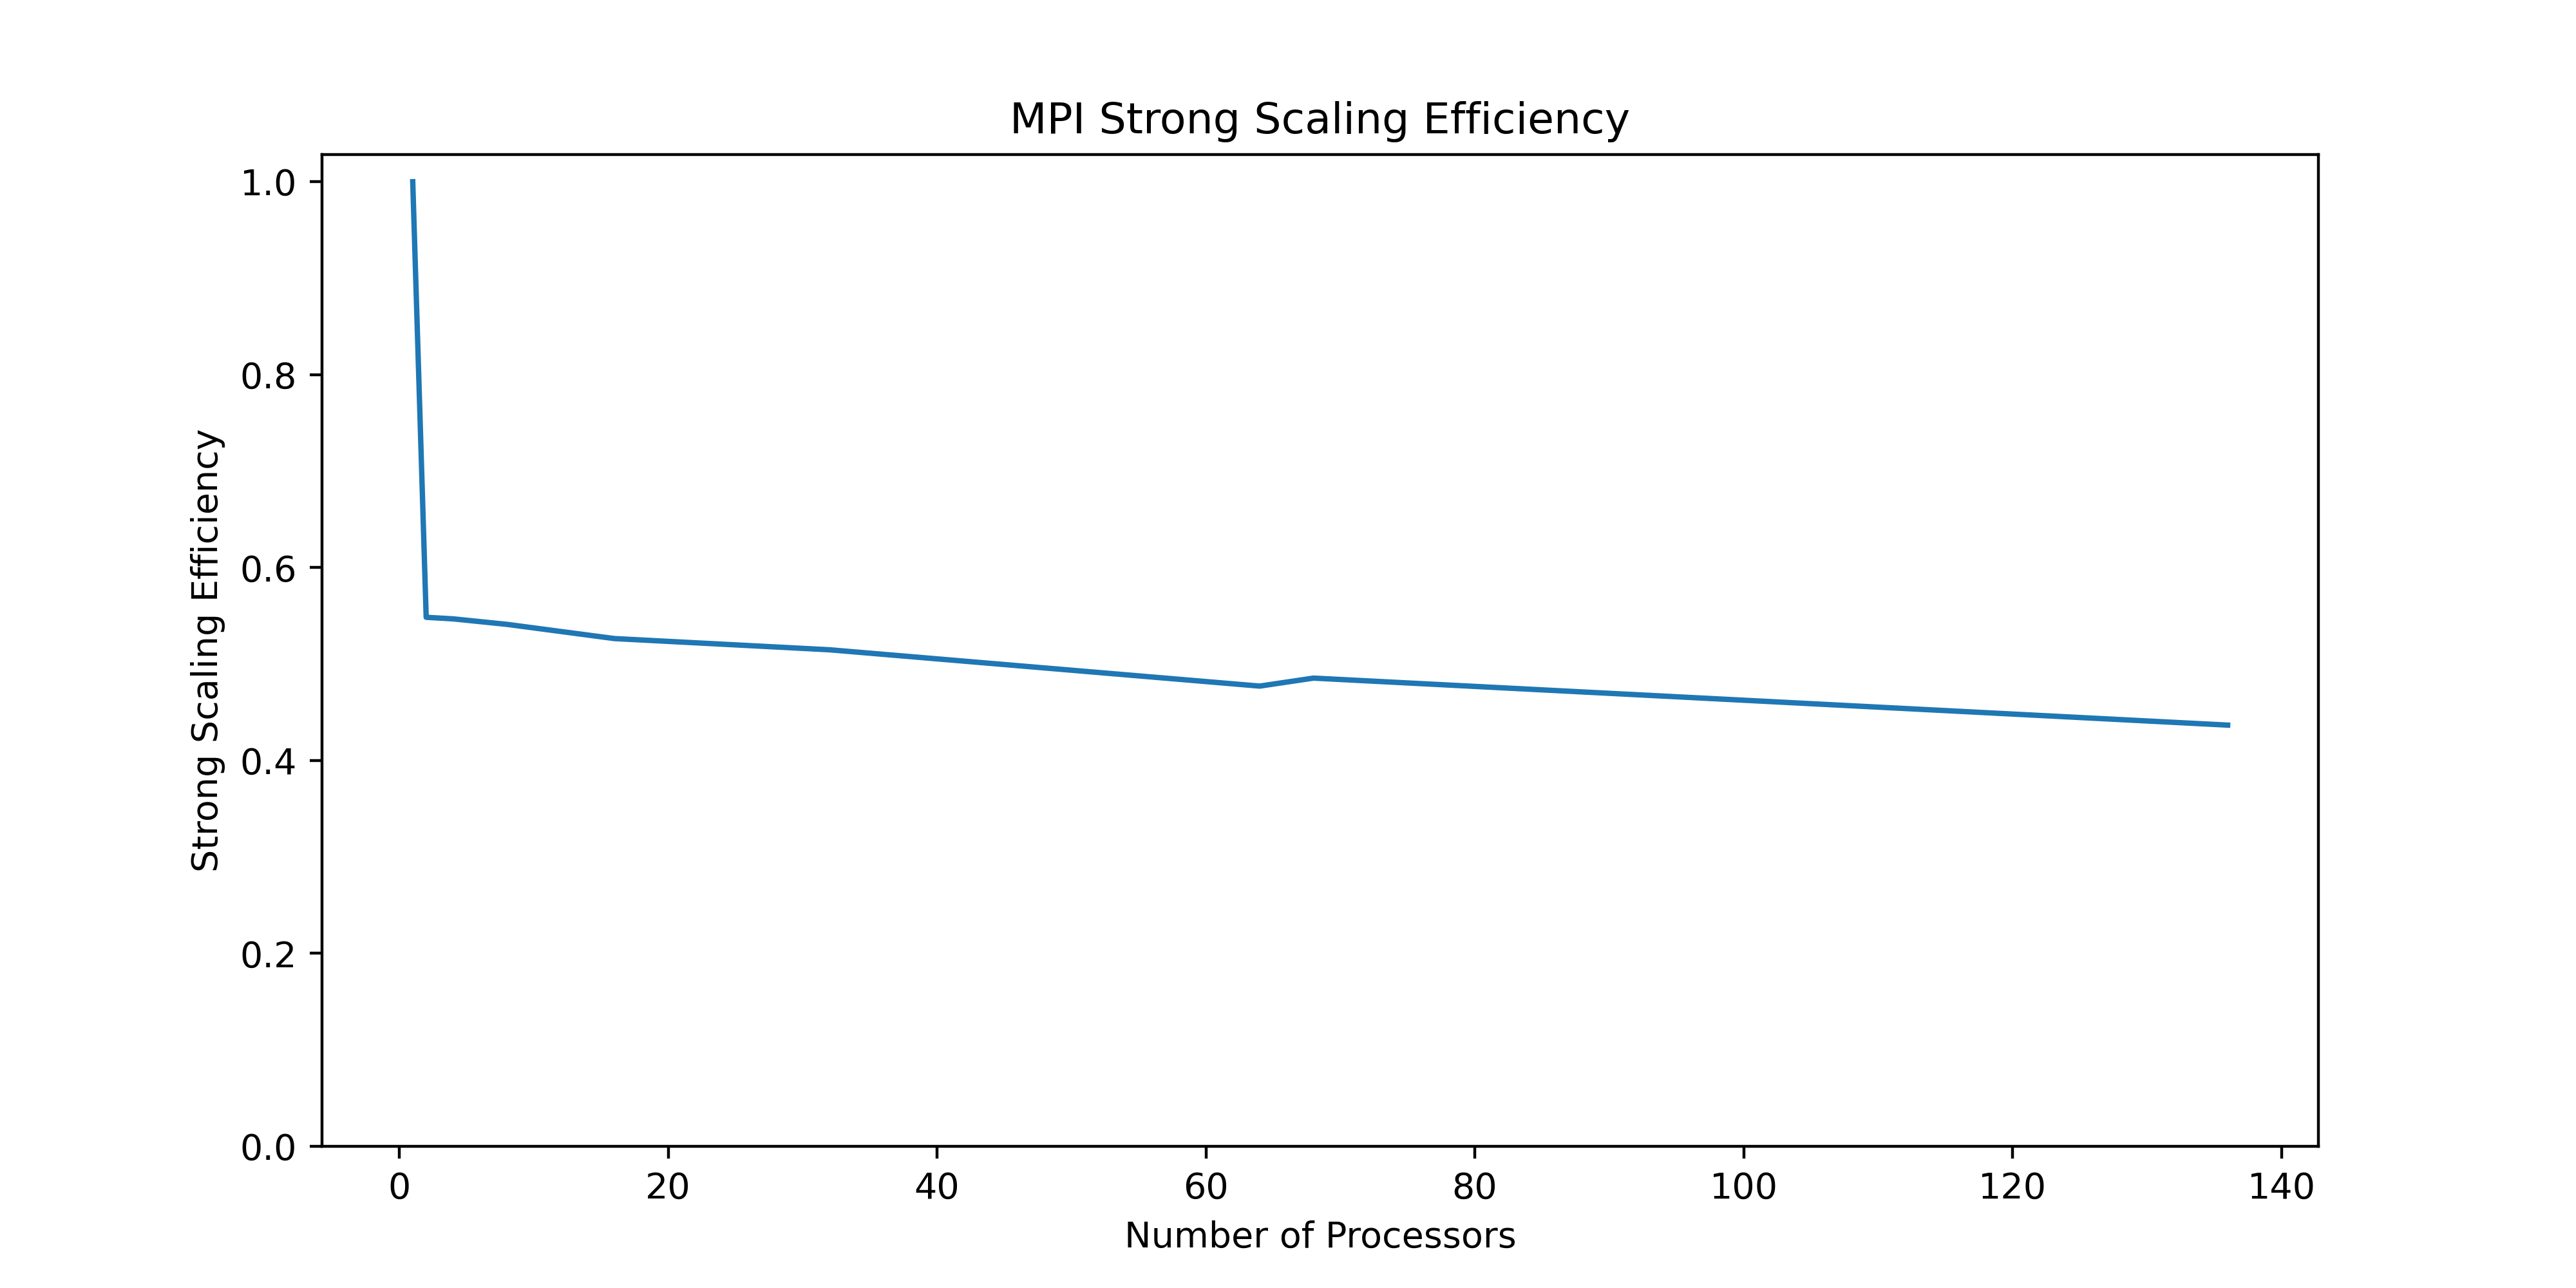
\includegraphics[width=6in]{figures/mpi_strong_scaling_efficiency.png}
	\caption{MPI Strong Scaling Efficiency}
	\label{fig:mpi-strong-scaling-efficiency}
\end{figure}

To see the results better, Figure \ref{fig:mpi-strong-scaling-efficiency} shows the strong scaling efficiency. There is a large dropoff in efficiency to 2 processors, giving 54.8\% efficiency. It sustains performance down to 43.7\% efficiency when all 136 cores are used. This is pretty low effiency, but considering that it is sustained, we deemed it scalable. This huge dropoff must have been due to the high communication overhead added on top of our synchronization overhead. We see later in our performance breakdown, that MPI communication overhead is indeed the main cause.

\begin{figure}[H]
	\centering
	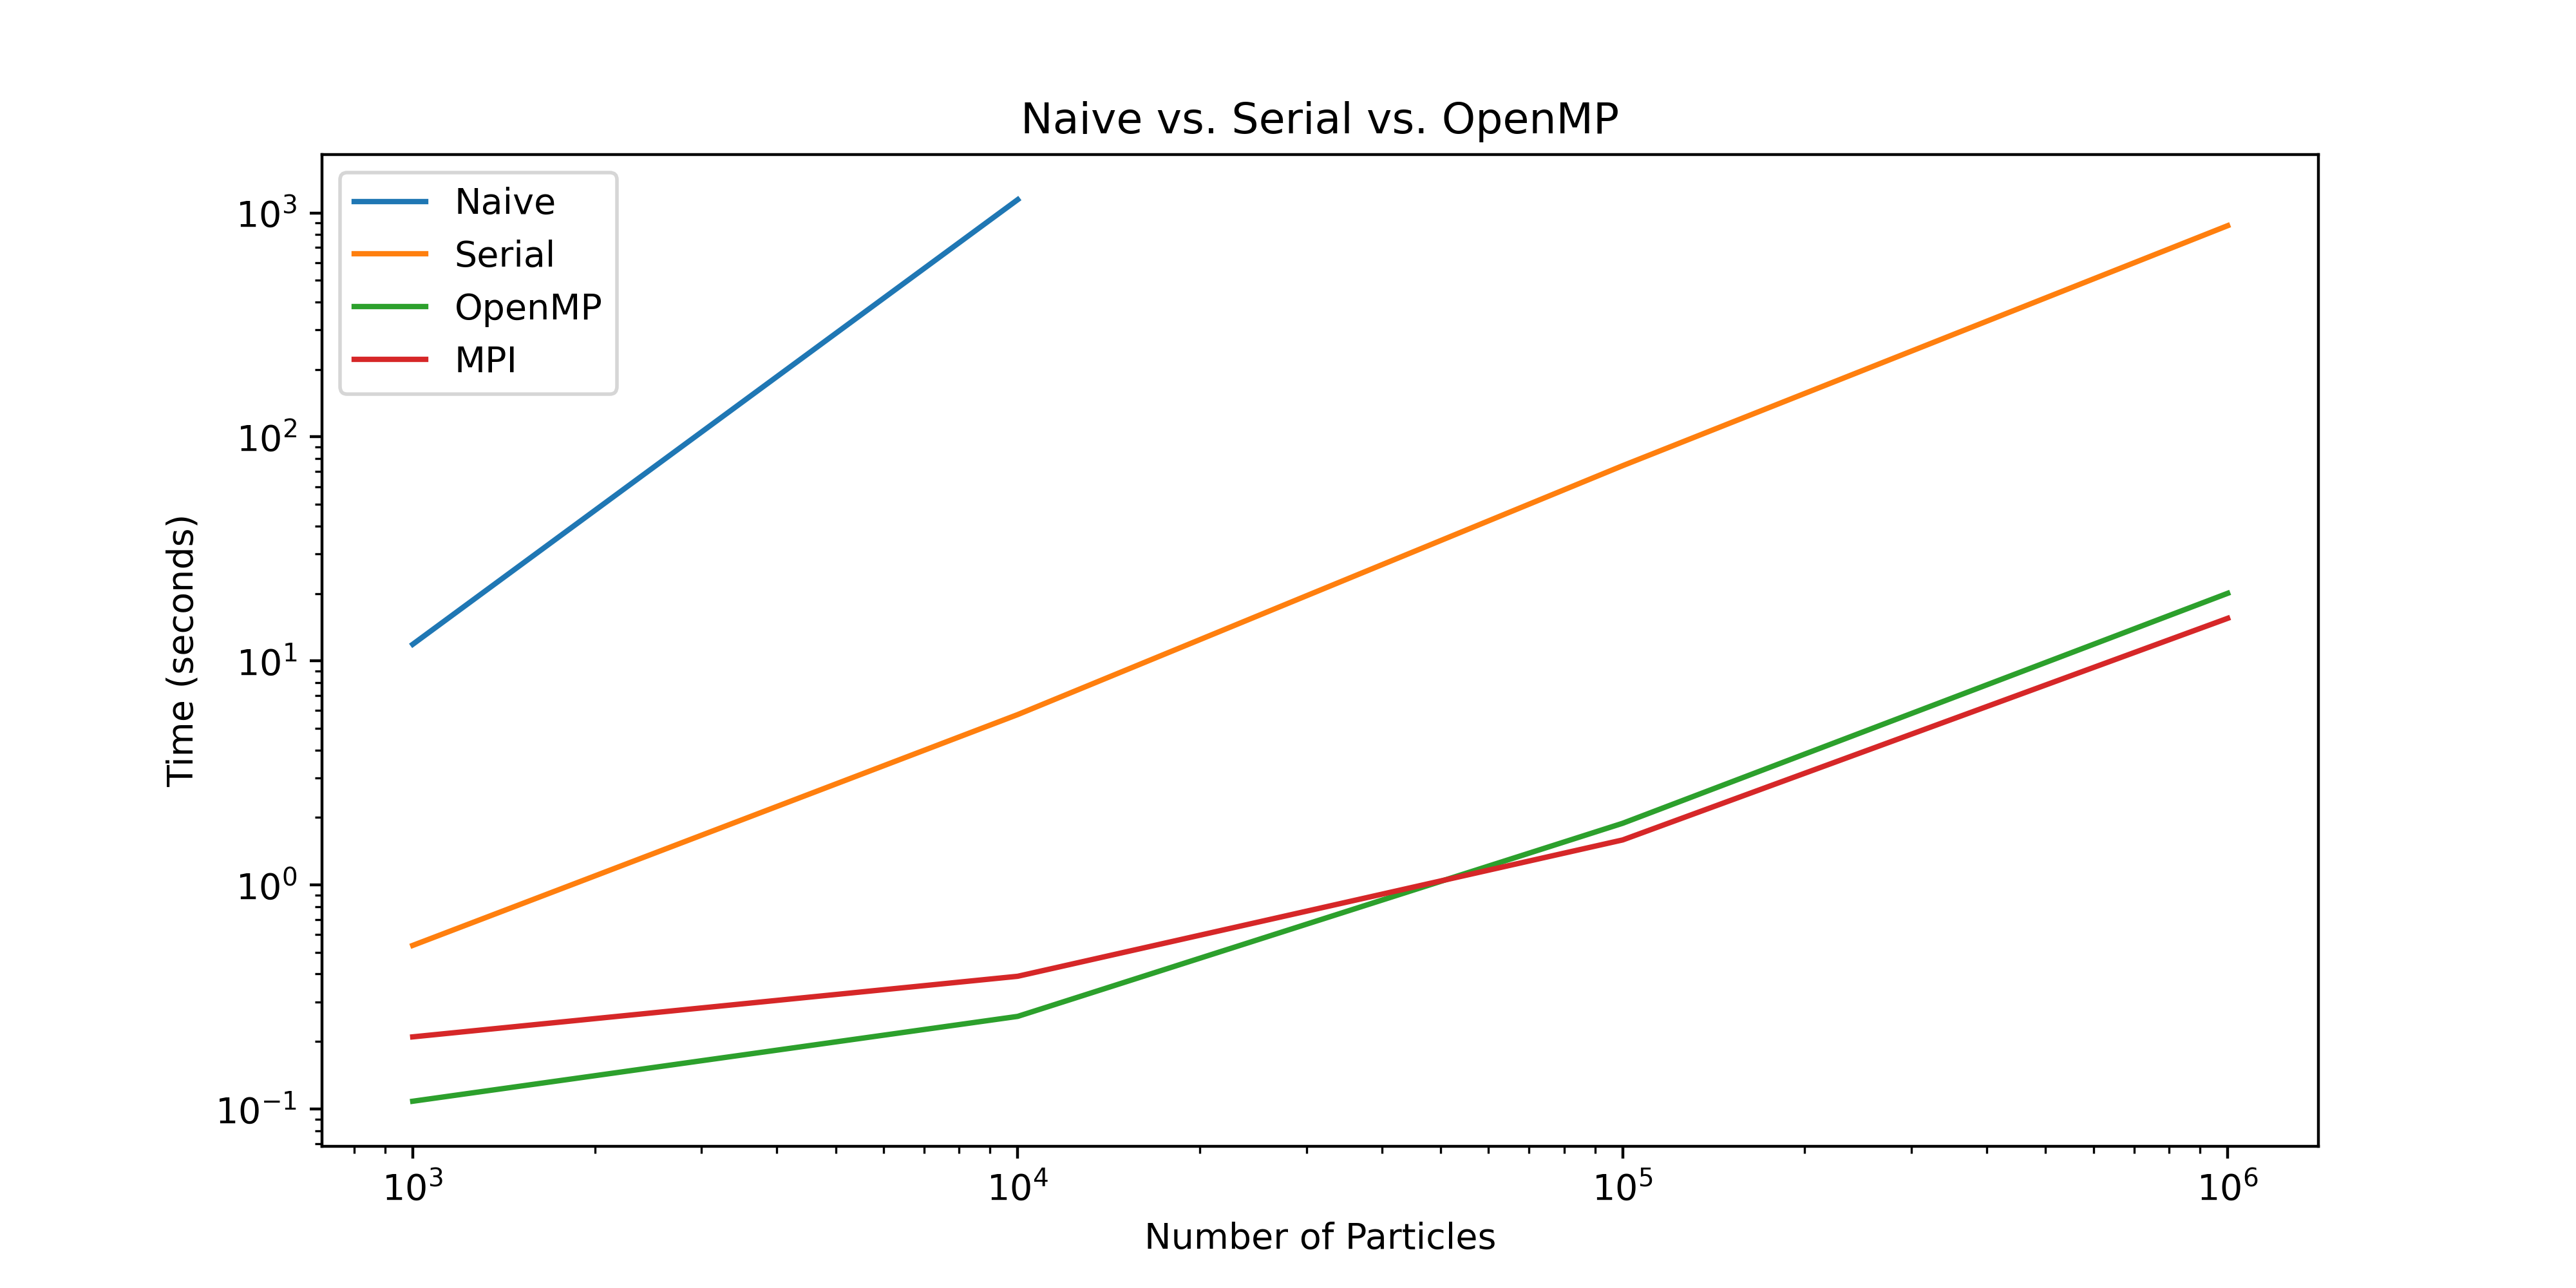
\includegraphics[width=6in]{figures/mpi_compared.png}
	\caption{Naive vs. Serial vs. OpenMP vs. MPI}
	\label{fig:mpi-compared}
\end{figure}

Figure \ref{fig:mpi-compared} shows the performance comparison between all of the other programming systems we have implemented so far for the $n$-body simulation.

\subsection{Performance Breakdown}

Profiling with MPI was difficult, as some of the profilers did not work smoothly with multiple nodes. We were able to successfully profile with Arm Performance Reports with limited configurations. Figure \ref{fig:mpi-profile-trace} shows a sample output of the trace. Embarrassingly, it shows that 98.8\% of our code is MPI bound, telling us that most of the time is spent in communication overheads. Due to the difficulty of debugging with MPI and working with distributed systems, we wish to improve this more if given more time and experience with MPI.

\begin{figure}[H]
	\centering
	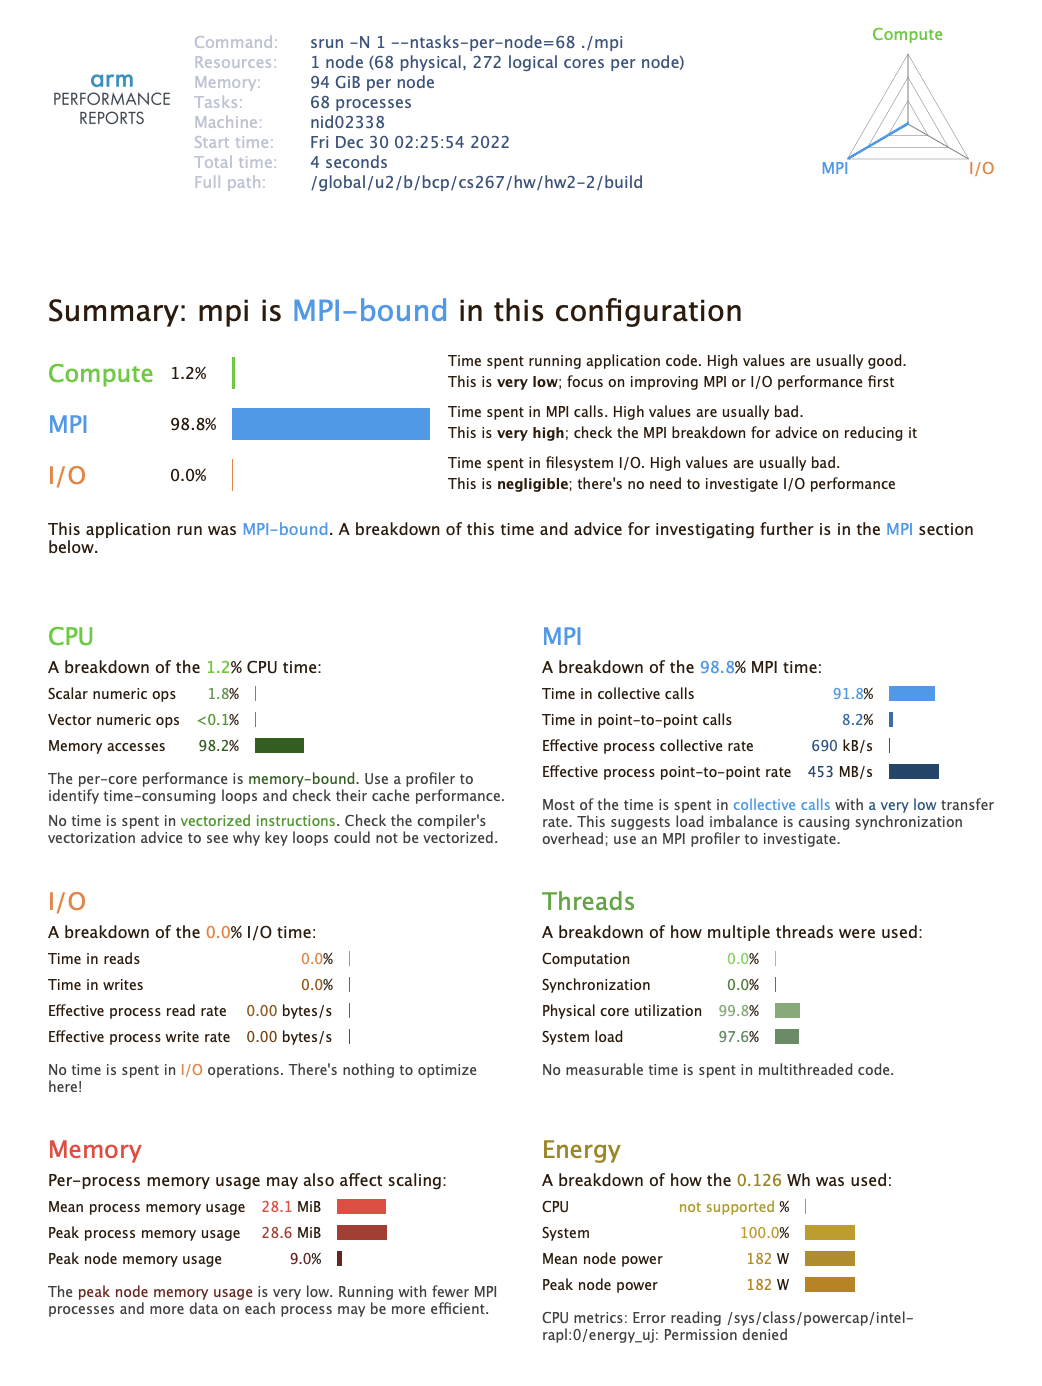
\includegraphics[width=6in]{figures/mpi_profile.png}
	\caption{Arm Performance Reports MPI Profile Trace}
	\label{fig:mpi-profile-trace}
\end{figure}

\section{Can We Do Better?}
Some design choices we made were mainly simple, to ease debugging and development. Along with the grid partitioning, we also had to be mindful of how we think about programming a MPMD (multiple program multiple data) model. Because the exact same code is being run at the same time, we had to make sure we also synchronize and think creatively how to distribute computation across partitions of data. The use of \verb|rank| was useful, and we figured out a way to make this scalable with various number of nodes and processes that MPI and the KNL nodes provide. We partitioned it such that each process or rank will be allocated a row of the grid space data structure. If we have less ranks than rows provided by the working set, we spill over and have ranks allocate more than one row for computation, denoted by \verb|leftover_processes|. Not proceeding with a rank to 2D mesh allocation may have affected performance, as load balancing could improve. With 2D, you could have more ranks do less computation, thus also potentially minimizing communication bottleneck between proceses.

Like the previous project, we computed the theoretical peak of our system on 2 nodes. The theoretical peak defined for our simulation can be derived as:
$$\frac{1.4 \times 10^9 \textrm{ instructions}}{\textrm{second}} * 136 \textrm{ cores} = 190.4 \textrm{ GFLOPS}$$

\begin{figure}[H]
	\centering
	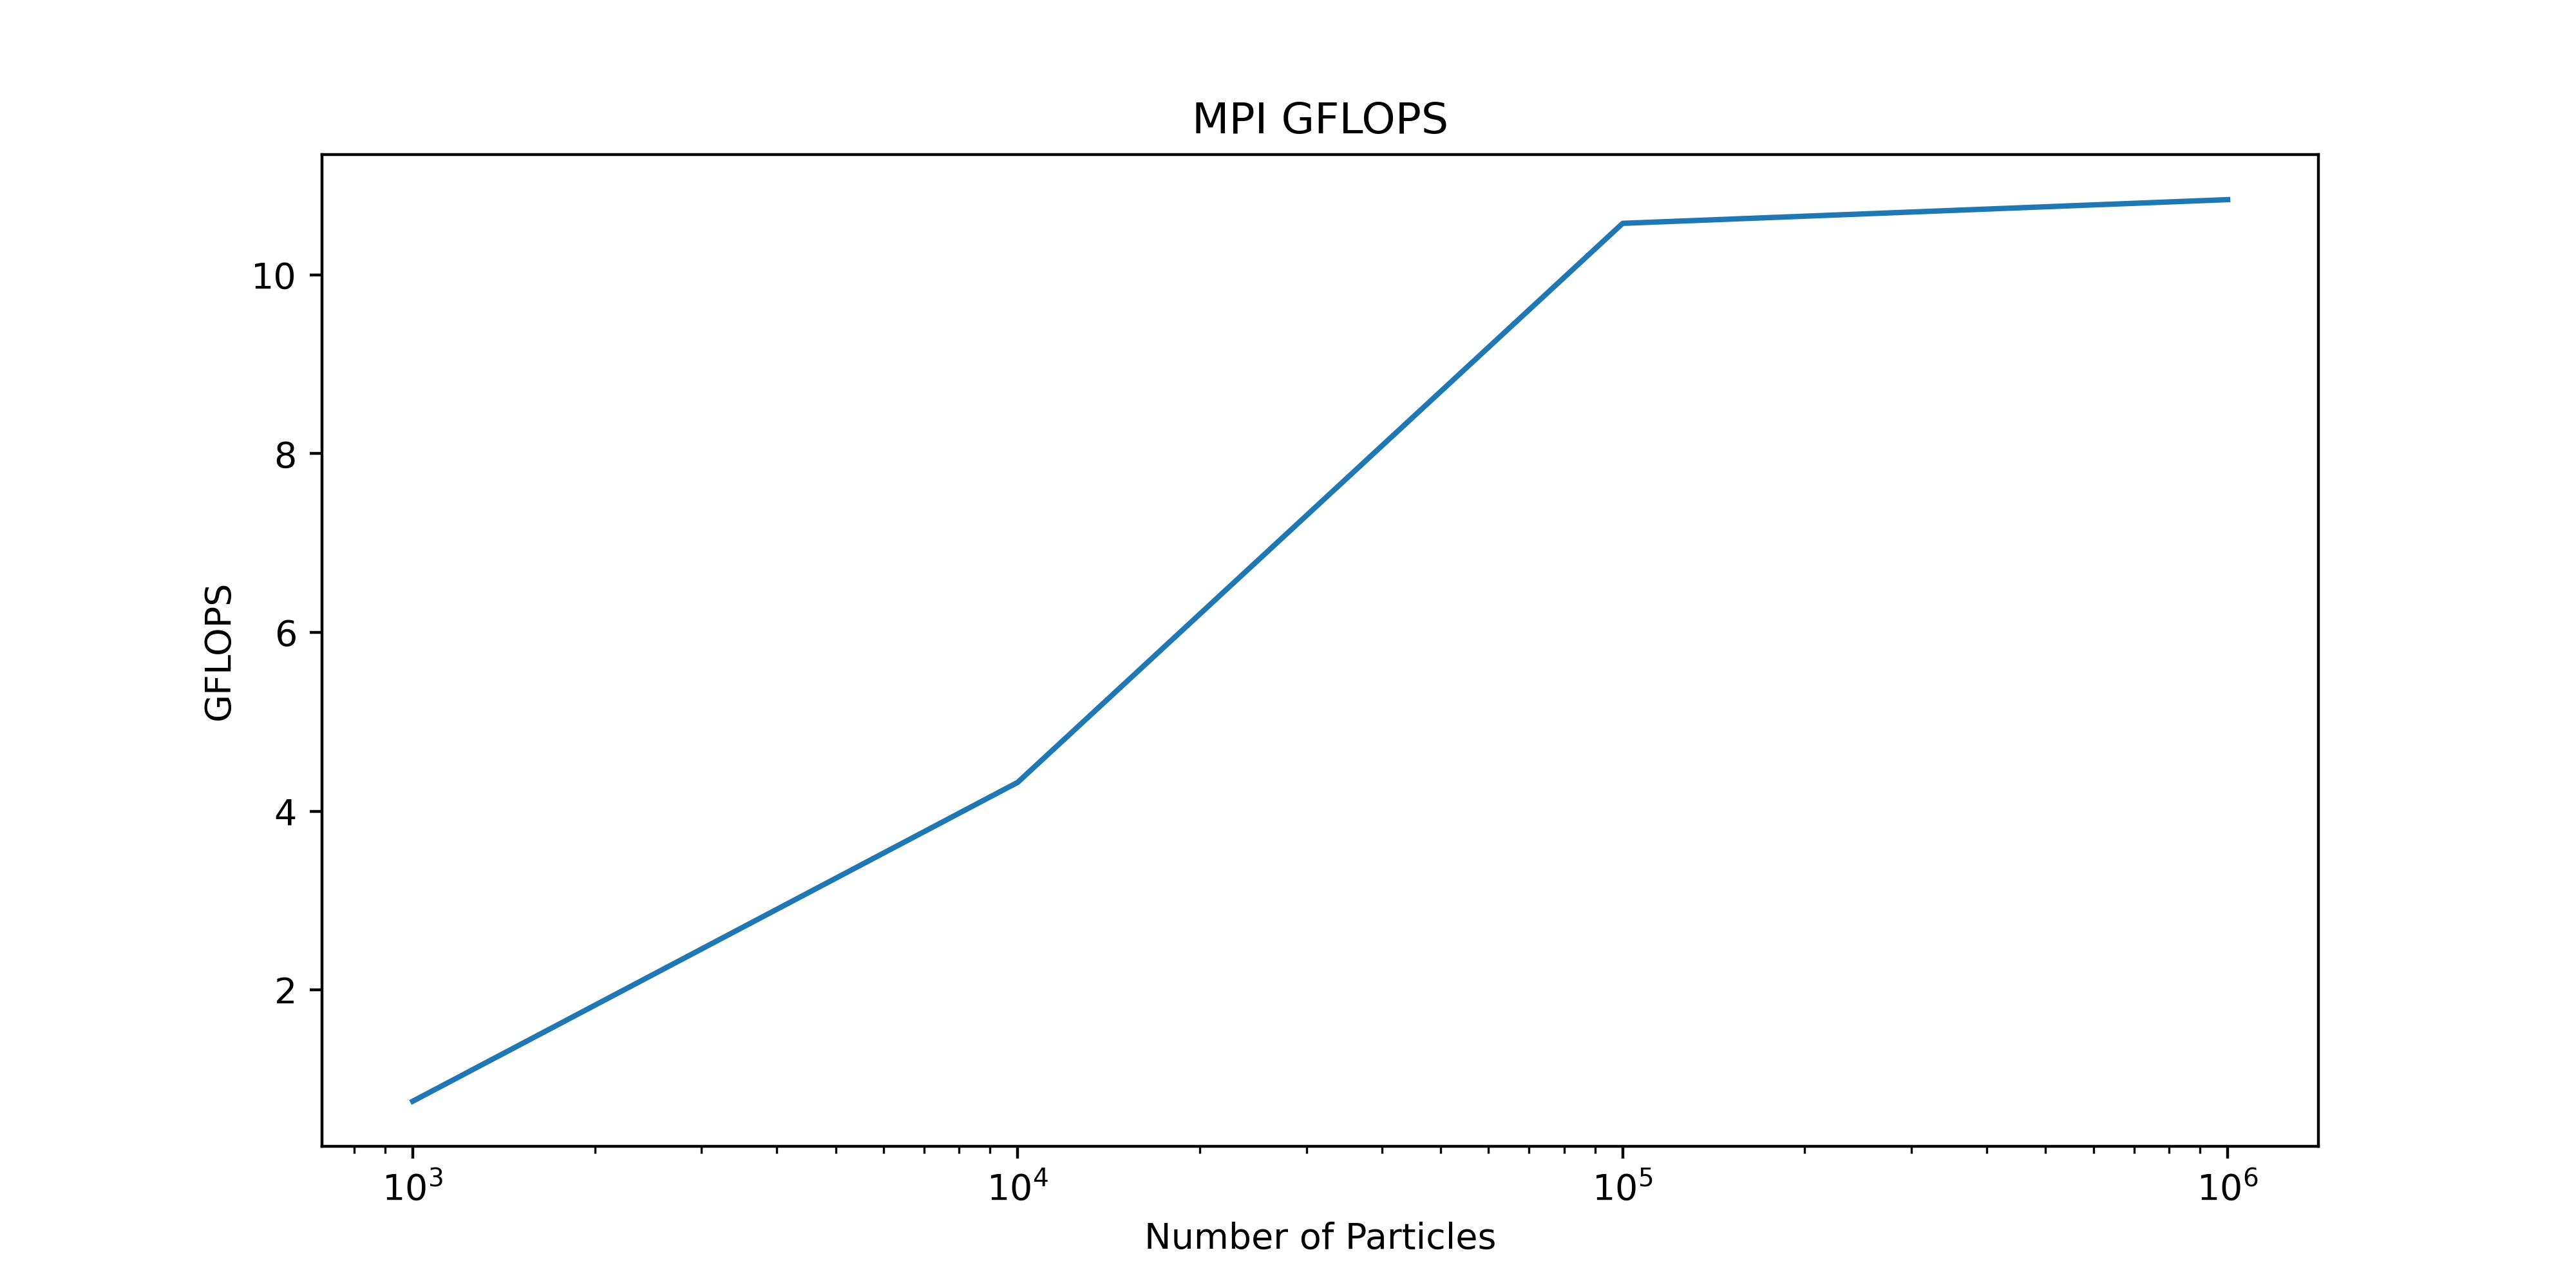
\includegraphics[width=6in]{figures/mpi_flops.png}
	\caption{MPI FLOPS}
	\label{fig:mpi-flops}
\end{figure}

When computing the performance, we see that we reach a peak of 10.84 GFLOPS, which is 5.7\% of theoretical peak. This is around $2\times$ worse than our OpenMP solution. Trying to make our simulation communication optimal was very difficult. In order to do substantially better, we have to consider not only synchronization and compute efficiency, but also communication bottlenecks as well. The only benefit that our code has over other methods, such as OpenMP, is that we can scale it beyond a single node. Our performance plot also shows that our simulation in MPI hits a ``roof" at around 11 GFLOPS. The slant indicates potentially our memory bound. When debugging performance, we could try to do higher particle count and aim to raise that roof as high as we can. The key and difficulty in this assignment seemed to be trying to hide the communication latencies, as we see from our embarassingly high MPI overhead.

\section{Contributions}
Everyone started off the exploration of MPI together. Andrew tried to divide columns of bins among each process while Brian and Xuan used a row approach. Brian was able to figure out how to add MPI directives to optimize code. Brian also figured out how to solve segmentation fault errors and finally put everything in working and presentable condition. In the end, Brian's approach was used as the final solution.

\bibliographystyle{ieeetr}
\bibliography{references}
\end{document}